\section{Signale im Zeitbereich}
  \subsection{Signalcharakterisierung}
  \begin{enumerate}
      \item{\textbf{Kontinuierlich \hfill $\longleftrightarrow$ \hfill Diskret}}
      \item{\textbf{Deterministisch \hfill $\longleftrightarrow$ \hfill Stochastisch}}\\
          Deterministische Signale sind mathematisch beschreibbar, im gegensatz
          zu stochastischen Signalen die dem Zufall unterworfen sind
      \item{\textbf{Periodisch \hfill $\longleftrightarrow$ \hfill Aperiodisch}}\\
          \begin{mdframed}[style=exercise]
              periodisch wenn, $x(t)=x(t+T_p)$ gilt.

              $T_p$ hei{\ss}t Grundperiode.
          \end{mdframed}
      \item{\textbf{Gerade \hfill $\longleftrightarrow$ \hfill Ungerade:}}\\
          \begin{mdframed}[style=exercise,frametitle=Zerlegung des Signals:]
              - gerader Anteil: \[x_G=\frac{1}{2}\left[x(t)+x(t-1)\right]\]
              - ungerader Anteil: \[x_U=\frac{1}{2}\left[ x(t)-x(-t) \right]\]
          \end{mdframed}
          \begin{center}
              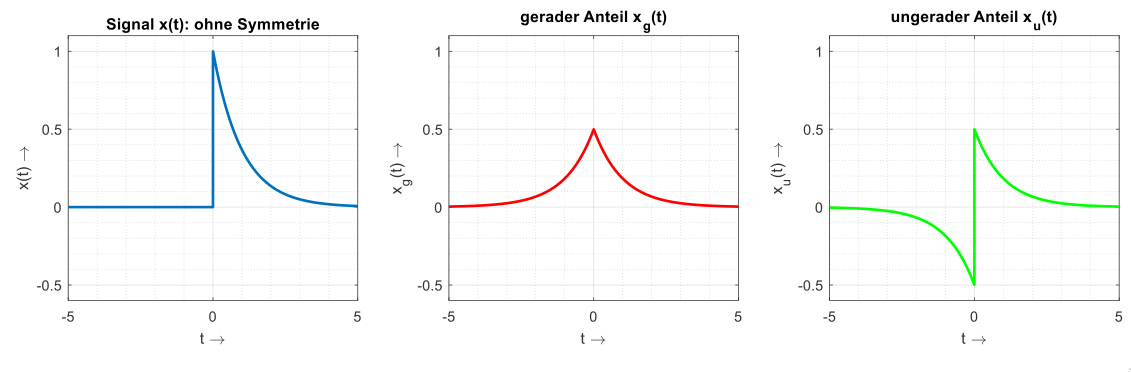
\includegraphics[width=0.43\textwidth]{gerade_ungerade_signal}
          \end{center}
      \item{\textbf{Energiesignal \hfill $\longleftrightarrow$ \hfill Leistungssignal}}
          \begin{mdframed}[style=exercise]
              Energie: \[E_x=\int_{t=-\infty}^{+\infty}\lvert x(t)\rvert^2 dt\]
              Leistung: \[P_x=\lim_{T\to\infty}\frac{1}{2T}\int_{-T}^{+T}\lvert x(t)\rvert^2 dt\]
          \end{mdframed}
      \item{\textbf{Korrelation}}\\
          Die Korrelationsfunktion ist eine Ma{\ss} f\"ur die \"Ahnlichkeit
          zweier deterministischer Energiesignale.
          \begin{mdframed}[style=exercise,frametitle=Korrelationsfunktion]
              \[
                  r_{xy}(\tau) = \int_{-\infty}^{\infty}x(t)\cdot y(t+\tau)dt
              \]
          \end{mdframed}
      \item{\textbf{Transformation}}\\
          Signale k\"onnenn modifiziert werden durch Ver\"andern der
          unabh\"angigen Variablen:
          \begin{itemize}
              \item Zeitverschiebung
              \item Zeitdehnung und Stauchung
              \item Zeitumkehr
          \end{itemize}
          \begin{mdframed}[style=exercise]
              \[
                  x_2(t) = x_1(-at+b)
              \]
          das Argument von $x_1(\tau)$ stellt eine Abbildung $t\rightarrow\tau$
          dar, daher bewirkt
          \begin{itemize}
              \item{$+b / -b\ (b > 0)$ eine Verschiebung von $x_1(\tau)$ nach links / rechts}

              \item{eine Multiplikation mit a / Division durch a $(a>1)$ eine Stauchung /
                  Streckung von $x_1(\tau)$}

              \item{Multiplikation mit -1 eine Spiegelung an der Ordinatenachse}
          \end{itemize}
          Die Reihenfolge der Schritte ist nicht \textbf{EGAL}:\\
          \color{red}{erst Verschieben um $b$, dann Skalieren/Invertieren mit $-a$}
          \end{mdframed}
  \end{enumerate}
  \subsection{Elementarsignale}
  \begin{mdframed}[style=exercise]
      \begin{itemize}
          \item{Sprungfunktion $\varepsilon$}
          \[ \varepsilon(t) =
             \begin{cases}
                 0 & \text{f\"ur } t < 0\\
                 1 & \text{f\"ur } t \geq 0
             \end{cases}
          \]
          \item{Dirac $\delta$}
          \[
              \int_{t=-\infty}^{\infty} \delta(t)dt = 1
          \]
          Eigenschaften:
          \begin{itemize}
              \item{H\"ohe unendlich}
              \item{Fl\"ache = 1}
              \item{Zusammenhang mit Sprungfunktion}\\
                  $\int_{\tau=-\infty}^{t}\delta(\tau)d\tau =
                  \varepsilon(t)$ bzw.  $\dfrac{d}{dt}\varepsilon(t) =
                  \delta(t)$
              \item{Ausblendeigenschaft}
                  \[
                      \delta(t-t_0)\cdot y(t) = \delta(t-t_0)\cdot y(t_0)
                  \]
              \item{Zeitskalierung: }
                  $\delta(at)=\frac{1}{\lvert a\rvert}\delta(t)$
          \end{itemize}
          \item{Dreieckimpuls $\Lambda$}
          \[ \Lambda(t) =
             \begin{cases}
                 0 & \text{f\"ur } \vert t\rvert > 1\\
                 1 & \text{f\"ur } \vert t\rvert \leq 1
             \end{cases}
          \]
          \item{Rechteckfunktion $rect$}
          \[ rect(t) =
             \begin{cases}
                 1 & \text{f\"ur } \vert t\rvert \leq \frac{1}{2}\\
                 0 & \text{f\"ur } \vert t\rvert > \frac{1}{2}
             \end{cases}
          \]
          Darstellbar durch:\\ $rect(t) = \varepsilon\cdot\left( t+\frac{1}{2} \right)-\varepsilon\cdot\left( t-\frac{1}{2} \right)$
          \item{Komplexe Exponentialfunktion}
          \[ \Lambda(t) =
             \begin{cases}
                 0 & \text{f\"ur } \vert t\rvert > 1\\
                 1 & \text{f\"ur } \vert t\rvert \leq 1
             \end{cases}
          \]
      \end{itemize}
  \end{mdframed}
